% =============================================================================
% COPYRIGHT AND DISCLAIMER
% =============================================================================
% This file is provided as a convenience template for competition participants.
% By using it, you accept full responsibility for compliance with all applicable
% copyright, licensing, and usage rules of the Association for Computing
% Machinery (ACM) and of any LaTeX packages you load (including, without
% limitation, the "acmart" document class and related ACM materials).
%
% Consult ACM's official publication, template, and copyright policies before
% using this setup for any purpose other than this competition. Do not assume
% that this template may be reused, redistributed, or submitted elsewhere
% without independently verifying ACM's current rules.
%
% Use of the "acmart" class, the "sigconf" option, or ACM-style formatting in
% this template does NOT mean that this report, this competition, its organizers,
% or any resulting PDF is sponsored, endorsed, affiliated with, or published by
% ACM. ACM trademarks and branding remain the property of ACM.
%
% Template packages live in preamble.tex.
% Citations live in main.bib. Edit this file with your paper content.
% =============================================================================

\documentclass[sigconf]{acmart}
% =============================================================================
% Template setup — participants normally do not edit this file.
% Author content belongs in main.tex; citations belong in main.bib.
% \documentclass lives in main.tex so Overleaf does not treat this file as root.
% =============================================================================

% --- Competition / non-ACM-submission friendly rights metadata ------------
\setcopyright{none}
\settopmatter{printacmref=false}
\acmConference[Kaggle Competition]{Filament Segmentation Challenge}{2026}{\href{https://www.kaggle.com/competitions/filament-segmentation-2026}{kaggle.com/competitions/filament-segmentation-2026}}
\acmBooktitle{Competition Report}
\acmDOI{}
\acmISBN{}

% --- Author guidance text --------------------------------------------------
% \guide{...} is gray italic while \guideStyletrue; omitted from the PDF if false.
% Flip the switch in main.tex after % =============================================================================
% Template setup — participants normally do not edit this file.
% Author content belongs in main.tex; citations belong in main.bib.
% \documentclass lives in main.tex so Overleaf does not treat this file as root.
% =============================================================================

% --- Competition / non-ACM-submission friendly rights metadata ------------
\setcopyright{none}
\settopmatter{printacmref=false}
\acmConference[Kaggle Competition]{Filament Segmentation Challenge}{2026}{\href{https://www.kaggle.com/competitions/filament-segmentation-2026}{kaggle.com/competitions/filament-segmentation-2026}}
\acmBooktitle{Competition Report}
\acmDOI{}
\acmISBN{}

% --- Author guidance text --------------------------------------------------
% \guide{...} is gray italic while \guideStyletrue; omitted from the PDF if false.
% Flip the switch in main.tex after % =============================================================================
% Template setup — participants normally do not edit this file.
% Author content belongs in main.tex; citations belong in main.bib.
% \documentclass lives in main.tex so Overleaf does not treat this file as root.
% =============================================================================

% --- Competition / non-ACM-submission friendly rights metadata ------------
\setcopyright{none}
\settopmatter{printacmref=false}
\acmConference[Kaggle Competition]{Filament Segmentation Challenge}{2026}{\href{https://www.kaggle.com/competitions/filament-segmentation-2026}{kaggle.com/competitions/filament-segmentation-2026}}
\acmBooktitle{Competition Report}
\acmDOI{}
\acmISBN{}

% --- Author guidance text --------------------------------------------------
% \guide{...} is gray italic while \guideStyletrue; omitted from the PDF if false.
% Flip the switch in main.tex after \input{preamble}.
%
% Do not use \guide{...} for \email{...}.
\usepackage{xcolor}
\newif\ifguideStyle
\guideStyletrue
\newcommand{\guide}[1]{%
  \ifguideStyle
    {\color{gray!65}\itshape #1}%
  \fi
}

% --- Math ------------------------------------------------------------------
% Do NOT load amssymb (or amsfonts): acmart already loads newtxmath, which
% defines the same symbols (e.g. \Bbbk) and causes a conflict on Overleaf.
% amsmath is already provided by acmart; mathtools extends it.
\usepackage{mathtools}

% --- Figures ---------------------------------------------------------------
% graphicx is already loaded by acmart
\usepackage{subcaption}

% --- Tables ----------------------------------------------------------------
% booktabs is already loaded by acmart
\usepackage{tabularx}
\usepackage{multirow}

% --- Bibliography style is set in main.tex (ACM-Reference-Format) ---------
.
%
% Do not use \guide{...} for \email{...}.
\usepackage{xcolor}
\newif\ifguideStyle
\guideStyletrue
\newcommand{\guide}[1]{%
  \ifguideStyle
    {\color{gray!65}\itshape #1}%
  \fi
}

% --- Math ------------------------------------------------------------------
% Do NOT load amssymb (or amsfonts): acmart already loads newtxmath, which
% defines the same symbols (e.g. \Bbbk) and causes a conflict on Overleaf.
% amsmath is already provided by acmart; mathtools extends it.
\usepackage{mathtools}

% --- Figures ---------------------------------------------------------------
% graphicx is already loaded by acmart
\usepackage{subcaption}

% --- Tables ----------------------------------------------------------------
% booktabs is already loaded by acmart
\usepackage{tabularx}
\usepackage{multirow}

% --- Bibliography style is set in main.tex (ACM-Reference-Format) ---------
.
%
% Do not use \guide{...} for \email{...}.
\usepackage{xcolor}
\newif\ifguideStyle
\guideStyletrue
\newcommand{\guide}[1]{%
  \ifguideStyle
    {\color{gray!65}\itshape #1}%
  \fi
}

% --- Math ------------------------------------------------------------------
% Do NOT load amssymb (or amsfonts): acmart already loads newtxmath, which
% defines the same symbols (e.g. \Bbbk) and causes a conflict on Overleaf.
% amsmath is already provided by acmart; mathtools extends it.
\usepackage{mathtools}

% --- Figures ---------------------------------------------------------------
% graphicx is already loaded by acmart
\usepackage{subcaption}

% --- Tables ----------------------------------------------------------------
% booktabs is already loaded by acmart
\usepackage{tabularx}
\usepackage{multirow}

% --- Bibliography style is set in main.tex (ACM-Reference-Format) ---------

% Added for this report: the pipeline diagram, and keeping figures ahead of the
% Acknowledgment section.
\usepackage{tikz}
\usetikzlibrary{arrows.meta,calc}
\usepackage{placeins}

% Guide styling: \guideStyletrue = show gray italic hints; \guideStylefalse = omit them
% \guideStyletrue
\guideStylefalse

\begin{document}

\title[Detector-Guided Fusion for Filament Segmentation]{Detector-Guided Fusion of a U-Net and YOLO11 Detectors for Filament Instance Segmentation}
\subtitle{A Solution to the Solar Filament Segmentation Challenge 2026} % DO NOT CHANGE

\author{Amey Pawar}
\affiliation{%
\city{Mumbai}
\country{India}
}
\email{ameypawar1237@gmail.com}

\begin{abstract}
This report describes our solution to the Solar Filament Segmentation Challenge~2026, a Kaggle competition on automatic segmentation of solar filaments in GONG H-$\alpha$ observations. A ResNet34 U-Net, applied to limb-darkening-corrected frames with eight-fold test-time augmentation, decides which pixels are filament. Three YOLO11 instance-segmentation detectors decide which pixels belong to the same filament and how confident each instance is, and the detections claim U-Net pixels in order of confidence. Scored against every annotator's view and compared with a cross-fitted, paired bootstrap over 144 validation observations, this fusion raises Panoptic Quality (PQ) from 0.371 for the U-Net with connected components to 0.421, and the public leaderboard score from 0.32 to 0.37. Retraining with another random seed moves PQ by up to 0.010, as much as any U-Net variant we tried. A third of the remaining misses are near-misses in which annotators outline faint segments that the network scores below 0.3, and another third are filaments the detectors find but score below the cut-off, typically ones that not every annotator draws.
\end{abstract}

\maketitle

% ==================================== %
%             INTRODUCTION             %
% ==================================== %
\section{Introduction}
This report goes over the details of our submitted solution to the Solar Filament Segmentation Challenge~2026 \cite{filament-segmentation-2026}. The challenge, launched on July~10,~2026, is organized by the Earth-Space AI Research (ESAIR) Lab\footnote{\href{https://www.esairlab.com/home}{www.esairlab.com/}}. This challenge utilizes the MAGFiLO dataset for evaluation of the segmentation algorithms \cite{ahmadzadeh2024dataset}. Earlier deep-learning work on H$\alpha$ filaments used semantic U-Nets \cite{zhu2019filament,zhu2025flatunet} or instance segmentation with Mask R-CNN \cite{ahmadzadeh2019filament} and CondInst \cite{guo2022filament}; Diercke et al.\ \cite{diercke2024filament} paired a YOLOv5 detector with a U-Net, using the detector's boxes to train the U-Net. We pair the two at inference instead. Our solution separates two questions that one model answers poorly together: a U-Net \cite{ronneberger2015unet} decides \emph{which pixels} are filament at full resolution, and instance detectors decide \emph{which pixels form one filament} and how likely it is to appear in an annotator's reference. We contribute a detector-guided fusion that adds 0.05 PQ over connected components, an evaluation protocol that matches the organisers' multi-annotator scoring and separates gains from noise, and an error analysis placing the remaining headroom in annotation ambiguity and seed variance.

% ==================================== %
%              METHODOLOGY             %
% ==================================== %
\section{Methodology}\label{sec:methodology}

\begin{figure*}[t]
\centering
\begin{tikzpicture}[
  box/.style={draw, rounded corners=2pt, align=center, font=\footnotesize, inner sep=2pt,
              minimum height=10mm},
  lane/.style={font=\footnotesize\itshape, anchor=west},
  arr/.style={-{Stealth[length=1.6mm]}, semithick}]
\node[box, text width=25mm] (data) at (0,0) {MAGFiLO: 707 labelled\\observations, split by day:\\563 train, 144 val\\(two halves of 72);\\180 test frames};
\node[box, text width=20mm] (pre) at (3.0,0) {limb fit and\\limb-darkening\\correction; input:\\intensity, radius};
\node[box, text width=28mm] (unet) at (6.2,0.74) {U-Net, ResNet34 encoder:\\512$^2$ crops, one annotator\\view per obs., Dice + BCE};
\node[box, text width=22mm] (uinf) at (9.4,0.74) {tiled inference,\\8$\times$ flips/rotations:\\filament probability};
\node[box, text width=22mm] (ubin) at (12.05,0.74) {threshold 0.5,\\close ($r{=}3$), fill,\\inside the disk};
\node[box, text width=28mm] (det) at (6.2,-0.74) {3 YOLO11-seg detectors:\\every annotator view\\a sample, one class};
\node[box, text width=22mm] (dinf) at (9.4,-0.74) {instances with\\confidence, masks at\\full resolution};
\node[box, text width=22mm] (dmerge) at (12.05,-0.74) {merge detectors:\\IoU $>$ 0.5,\\mean confidence};
\node[box, text width=23mm, minimum height=25mm] (fuse) at (14.95,0) {fusion: in order of\\confidence, each\\detection scoring\\${\geq}\,0.30$ claims the\\unclaimed pixels in\\its mask grown 4\,px;\\claims $<$ 200\,px are\\dropped $\rightarrow$ one RLE\\mask per filament};
\node[lane] at (4.6,1.47) {U-Net: which pixels are filament};
\node[lane] at (4.6,-1.47) {detectors: which pixels form one filament};
\draw[arr] (data) -- (pre);
\draw[arr] (pre.east) -- ++(0.2,0) |- (unet.west);
\draw[arr] (pre.east) -- ++(0.2,0) |- (det.west);
\draw[arr] (unet) -- (uinf);
\draw[arr] (uinf) -- (ubin);
\draw[arr] (det) -- (dinf);
\draw[arr] (dinf) -- (dmerge);
\draw[arr] (ubin.east) -- ++(0.2,0) |- ($(fuse.west)+(0,0.74)$);
\draw[arr] (dmerge.east) -- ++(0.2,0) |- ($(fuse.west)-(0,0.74)$);
\end{tikzpicture}
\caption{End-to-end pipeline, from the labelled data to the submitted masks. Training happens in the first box of each lane; the rest runs on every frame. The U-Net supplies full-resolution filament pixels, and the detectors decide which pixels form one filament and how confident it is.}
\label{fig:pipeline}
\end{figure*}

Fig.~\ref{fig:pipeline} shows the whole pipeline.

\paragraph{Data and sampling.} The training set has 707 observations (2011--2022, six GONG sites) with 1{,}154 annotator views: each observation is annotated by one to three people, and each filament is one polygon. We split by calendar day into 563 training observations (906 views) and 144 validation observations (248 views), so frames of the same day never straddle the split. The 180 test observations, whose labels are withheld, are used only for submissions. Validation is divided into two fixed halves of 72 observations: parameters are tuned on one half and scored on the other, results on all 144 are \emph{cross-fitted}, each half scored with the parameters chosen on the other, and the parameters we submit are re-chosen on all 144. The U-Net's per-epoch checkpoint scores used 48 observations of the tuning half. We did not use the public MAGFiLO release, which contains the test labels.

\paragraph{Pre-processing.} GONG frames carry a bright, smooth halo beyond the limb whose outer edge is itself a sharp circle, so over all 887 frames a thresholded disk has a radius a median 39 pixels larger than the limb's, and up to 148 pixels larger. We start from three candidate circles (an intensity threshold, a texture threshold, since the disk is textured and the halo smooth, and the standard GONG geometry), snap each to the sharpest radial edge along 720 rays, and keep the smallest circle most rays support. Dividing by the median radial intensity profile removes limb darkening. The input has two channels: corrected intensity and radial distance normalised to the limb.

\paragraph{U-Net.} A U-Net \cite{ronneberger2015unet} with an ImageNet-pretrained ResNet34 encoder \cite{he2016resnet} (segmentation\_models\_pytorch \cite{iakubovskii2019smp}) is trained on 512$\times$512 crops at native resolution, eight per observation per epoch, 70\% of them centred near an annotated filament. Augmentation is limited to flips, 90-degree rotations and brightness/contrast jitter, because resampling destroys structures a few pixels wide. The loss is soft Dice \cite{milletari2016vnet} plus binary cross-entropy; AdamW at $10^{-3}$ with a cosine schedule for 30 epochs, batch 16, one annotator's view per observation, on one T4 GPU. We keep the final-epoch weights. Inference blends overlapping 512-pixel tiles with a Hann window and averages the logits over the eight flips and rotations of the frame \cite{wang2019tta}.

\paragraph{Detectors.} YOLO \cite{redmon2016yolo} detectors predict boxes and, in their segmentation variants, a coarse mask per instance in one pass. We train YOLO11-seg models \cite{jocher2024yolo11} on the corrected frames as one class, with every annotator's view as a separate sample, so that confidence reflects how many annotators would draw a filament. Mosaic augmentation is off, since a filament's appearance depends on its position on the disk. The entry uses three of the five we trained: detector~1 (YOLO11s, 1024 pixels, 60 epochs), detector~2 (YOLO11m, 1280 pixels, 80 epochs) and detector~4 (YOLO11m, 1536 pixels, 80 epochs). Detector~3 (YOLO11s at 1280 pixels, another seed) and detector~5 (detector~2's recipe, another seed) did not help (Section~\ref{sec:evaluation}). Detections from different models whose masks overlap with IoU above 0.5 are merged: the most confident mask is kept and the score is the mean over the three models, counting a model that missed the filament as zero.

\paragraph{Fusion (post-processing).} (1) The U-Net probability is thresholded at 0.5, closed with a 3-pixel disk, hole-filled and restricted to the solar disk. (2) In descending order of confidence, each detection scoring at least 0.30 claims the not yet claimed foreground pixels inside its own mask, which the detector outputs at full resolution, grown by 4 pixels; one claim is one instance, even if it spans several foreground components. (3) Claims under 200 pixels are dropped, and so is foreground no detection claims. Instances never overlap; they take their boundaries from the full-resolution U-Net and their grouping and confidence from the detectors. The five parameters were tuned under the protocol above.

\paragraph{Final entries.} The \emph{validated} entry uses the models above, trained on the 563 training observations. The \emph{all-data} entry retrains the same recipes on all 707 observations, averaging four U-Nets (seeds 0--3) and two seeds of each detector, with the fusion parameters fixed from the validated entry. It cannot be validated, so it was submitted once as a sanity check.

\begin{figure*}[t]
\centering
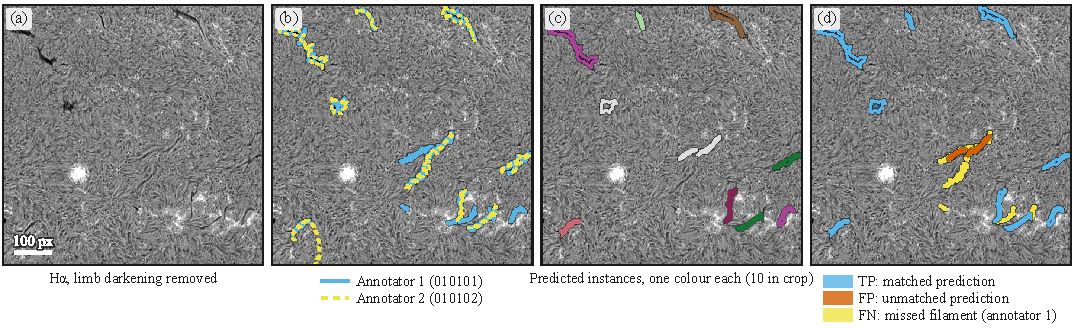
\includegraphics[width=\textwidth]{figures/fig_qualitative.pdf}
\caption{Segmentation example on a validation observation: (a) corrected H$\alpha$ crop; (b) each annotator's filaments; (c) predicted instances; (d) outcome against the first annotator: matched (TP), unmatched prediction (FP), missed filament (FN). The observation (20150518145654Bh, two annotators) has a per-observation PQ of 0.437, near the median. In the centre is a forked filament: annotator~1 draws its two branches separately, annotator~2 one path through it. The prediction covers only part of the upper branch, so against annotator~1 it is a near-miss, counted as both FP and FN, and the lower branch is missed.}
\label{fig:qualitative}
\end{figure*}

\begin{figure*}[t]
\centering
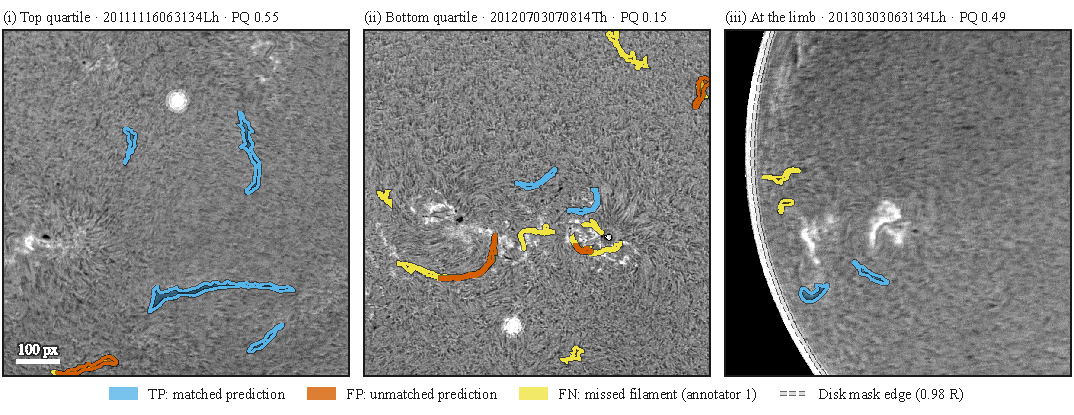
\includegraphics[width=\textwidth]{figures/fig_examples.pdf}
\caption{Three more validation observations, outcome against the first annotator as in Fig.~\ref{fig:qualitative}(d): (i) a top-quartile observation, where the predictions match; (ii) a bottom-quartile one, with near-misses (orange over yellow) and missed faint filaments; (iii) an observation at the limb, where the dashed line is the edge of the disk mask (0.98 of the fitted radius) beyond which nothing is predicted.}
\label{fig:examples}
\end{figure*}

% ==================================== %
%              EVALUATION              %
% ==================================== %
\section{Evaluation}\label{sec:evaluation}

\paragraph{Strategy.} The challenge scores Panoptic Quality \cite{kirillov2019panoptic}: for each annotator's view, a prediction matches a filament when their IoU exceeds 0.5, and true positives (TP), false positives (FP), false negatives (FN) and matched IoUs are summed over all views of all observations,
\begin{equation}
\mathrm{PQ}=\frac{\sum_{\mathrm{TP}}\mathrm{IoU}}{|\mathrm{TP}|+\frac12|\mathrm{FP}|+\frac12|\mathrm{FN}|}=\mathrm{SQ}\times\mathrm{RQ}.
\end{equation}
A prediction with IoU $\leq$ 0.5 adds both an FP and an FN, twice the cost of predicting nothing, and since every view counts, the annotators' consensus scores best; two MAGFiLO annotators agree with each other at only 0.343 PQ. Our scorer pools over views as the organisers' self-evaluation notebook does. Intervals come from bootstrap resampling of observations with their views kept together \cite{efron1993bootstrap}: 2{,}000 resamples per pipeline, 10{,}000 for paired differences. A change was kept if it improved PQ in at least 80\% of resamples, and submitted alone only if its 95\% interval excluded zero.

\begin{table}[t]
\caption{Progression. PQ on all 144 validation observations with its 95\% bootstrap interval, on the 72 held-out observations never used for tuning, and on the public leaderboard (two decimals, about half the test set).}
\label{tab:progress}
\footnotesize
\setlength{\tabcolsep}{4pt}
\begin{tabular}{@{}lccc@{}}
\toprule
Pipeline & Validation & Held-out & Public \\
\midrule
Intensity threshold, components & 0.125 & -- & 0.08 \\
U-Net, connected components & 0.371 [.348, .393] & 0.368 & 0.32 \\
Detectors 1, 2, 4 alone$^\ast$ & 0.383 [.360, .406] & 0.385 & -- \\
Fusion, detectors 1, 2$^\ast$ & 0.411 [.388, .433] & 0.419 & 0.36 \\
+ final-epoch U-Net$^\ast$ & 0.418 [.395, .440] & 0.428 & 0.37 \\
+ detector 4: validated$^\ast$ & \textbf{0.421} [.399, .443] & \textbf{0.433} & 0.37 \\
All-data entry & -- & -- & 0.37 \\
\bottomrule
\multicolumn{4}{@{}l}{\scriptsize $^\ast$Cross-fitted. The U-Net row's settings were tuned on the tuning half.}\\
\end{tabular}
\end{table}

\paragraph{Results.} Table~\ref{tab:progress} gives the progression. The model-free baseline matches filaments with reasonable masks (SQ 0.65) but finds few (RQ 0.20). Fusion adds 0.04--0.05 PQ to the U-Net, the largest gain after the U-Net itself, mostly through recognition (RQ 0.55 to 0.62, SQ 0.670 to 0.676). Neither half suffices alone: the three detectors' own masks reach 0.383, and the U-Net's pixels add 0.038 to them (95\% CI $+0.026$ to $+0.051$), raising SQ (0.651 to 0.676) and RQ (0.589 to 0.624). Eight-fold TTA added 0.009 on held-out data for an earlier U-Net (under our earlier single-annotator scorer) and 0.02 on the public board. The final-epoch U-Net weights beat the epoch selected on 48 observations by 0.007 (95\% CI $+0.004$ to $+0.011$); detector~4 adds 0.003, within the noise (gain in 82\% of resamples). Figs.~\ref{fig:qualitative} and~\ref{fig:examples} show examples, Table~\ref{tab:diag} the rubric's diagnostics and Fig.~\ref{fig:ioudice} the IoU and Dice distributions. Matched masks follow the annotations closely (median IoU 0.68, Dice 0.81); most of the loss is in recognition (recall 0.57), including near-misses whose extent the annotators draw differently. With one detection per instance, fragmentation and over-merging are rare: 45 of 1{,}857 annotated filament views are split across several predictions, and 59 of 1{,}543 predicted instance views span several annotated filaments.

\begin{table}[t]
\caption{Validated entry on 144 validation observations, pooled over all annotator views; 95\% bootstrap intervals in brackets.}
\label{tab:diag}
\footnotesize
\begin{tabular}{@{}lc@{}}
\toprule
Quantity & Value \\
\midrule
PQ$^\dagger$ & 0.424 [0.400, 0.446] \\
SQ (mean IoU of matches) & 0.676 [0.669, 0.683] \\
RQ & 0.627 [0.594, 0.657] \\
TP / FP / FN (instance views) & 1{,}066 / 477 / 791 \\
Precision / recall (hit rate) / miss rate & 0.691 / 0.574 / 0.426 \\
Matched IoU, median (IQR) & 0.683 (0.614--0.743) \\
Matched Dice, mean / median & 0.804 / 0.812 \\
One-to-many (fragmented filaments) & 45 \\
Many-to-one (over-merged predictions) & 59 \\
PQ by annotator group$^\ddagger$ & 0.400 to 0.493 \\
Runtime per 2048$^2$ frame$^\S$ & 6.6 s (all-data: 21 s) \\
\bottomrule
\multicolumn{2}{@{}p{\columnwidth}@{}}{\scriptsize $^\dagger$Settings tuned on these observations; cross-fitted PQ is 0.421. $^\ddagger$Views grouped by the first two digits of the annotator ID (6 groups, 15--120 views). $^\S$Mixed hardware: 0.3\,s pre-processing and 0.2\,s fusion (CPU), 4.0\,s per U-Net with TTA (Apple M5), 0.7\,s per detector (T4).}\\
\end{tabular}
\end{table}

\begin{figure}[t]
\centering
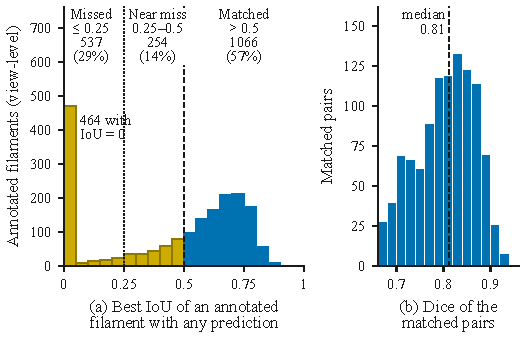
\includegraphics[width=\columnwidth]{figures/fig_iou_dice.pdf}
\caption{(a) Best IoU of each of the 1{,}857 annotated filament views with any prediction of the validated entry: 57\% matched, 14\% near-misses, 29\% missed (464 with no overlap). (b) Dice of the 1{,}066 matched pairs.}
\label{fig:ioudice}
\end{figure}

\paragraph{Where the errors are.} Fig.~\ref{fig:errors} breaks the errors down. A third of the 791 missed filament views (33\%) were found by a detector but scored below the 0.30 cut-off. The annotators disagree on these: only 30\% of the other annotators of the same observation drew them, against 72\% for the filaments we match. Lowering the cut-off adds about two FPs per TP, the break-even rate at this PQ. Another third (32\%) are near-misses (IoU 0.25--0.5): on average 86\% of the annotated pixels they leave out have U-Net probability below 0.3, so even a 0.3 threshold would recover at most 14\% of them. Only 9\% of misses have no detection at all, and missed filaments are smaller than matched ones (median 903 against 1{,}395 pixels). Half of the false positives (52\%) are near-misses, and on observations with several annotators 52\% of them match a filament that \emph{another} annotator drew.

\begin{figure}[t]
\centering
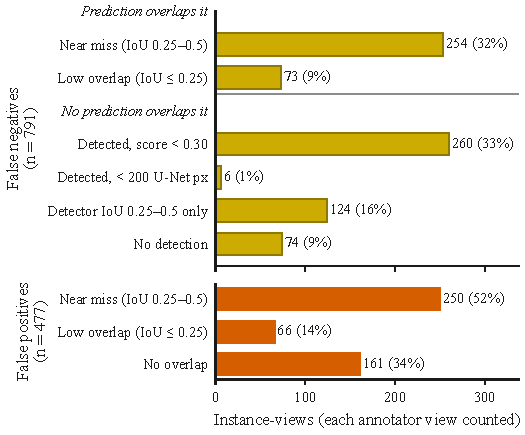
\includegraphics[width=\columnwidth]{figures/fig_errors.pdf}
\caption{Causes of false negatives and false positives (validated entry, per annotator view); a near-miss counts as both. ``Detector IoU 0.25--0.5 only'': a detection overlaps the filament poorly and no kept prediction does.}
\label{fig:errors}
\end{figure}

\paragraph{Seeds and negative results.} Fig.~\ref{fig:seeds} sets the variants we tried against seed-to-seed variation. Retraining the U-Net recipe with another seed lowered cross-fitted PQ by 0.007, and the strongest detector recipe by 0.010. The U-Net variants (all annotators' views instead of one per observation, the union of the annotators' masks, or a Tversky loss \cite{salehi2017tversky} weighting missed pixels above extra ones) score 0.407--0.412, no better than the recipe's second seed (0.410). Averaging three U-Nets other than run~3 gains 0.002 over a typical seed \cite{lakshminarayanan2017ensembles}, but no ensemble beats run~3. Post-processing changes were flat too: other thresholds, areas and cut-offs, looser merging, falling back to a detector's mask where the U-Net covers little of it, and keeping components no detection claims.

\begin{figure}[t]
\centering
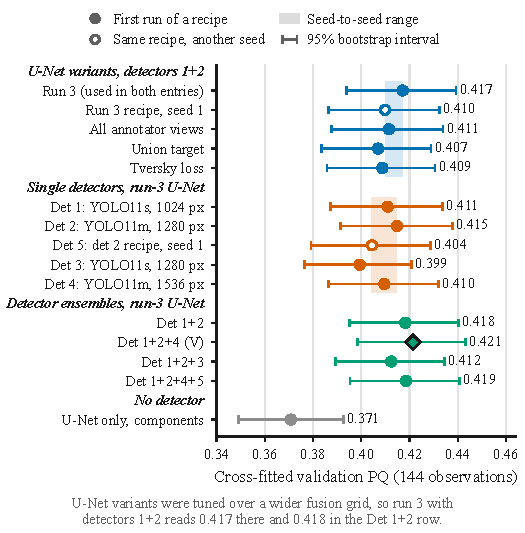
\includegraphics[width=\columnwidth]{figures/fig_seeds.pdf}
\caption{Cross-fitted validation PQ with each pipeline's own 95\% bootstrap interval; paired differences are much tighter (half-widths 0.004--0.010). Run~3 is the U-Net of both entries, V the validated entry.}
\label{fig:seeds}
\end{figure}

\paragraph{Validation versus leaderboard.} Validation PQ runs about 0.05 above the public score, and we could not pin the gap down. Temporal proximity does not explain it (test and validation observations are a median 2.0 and 2.1 days from the nearest training one), and reweighting validation to the test set's years or sites moves PQ by at most 0.003. Candidates are the test set's annotators, since the same predictions score 0.400 to 0.493 against different annotator groups, and noise: the public board scores about 90 observations, to two decimals.

\paragraph{Strengths, weaknesses and improvements.} The fusion is simple and transparent: each instance comes from one confident detection, so fragmentation and over-merging stay rare, and boundaries keep the U-Net's full resolution. Its weaknesses mirror the labels: near-misses and filaments only some annotators draw are disagreements between annotators as much as model errors, and seed variance is as large as most changes. Promising directions are a soft multi-annotator target that models filament extent, larger seed ensembles with calibrated instance scores, and a full-resolution refinement of faint filament ends. Code, every reported number, the trained weights and a reproduction notebook: \url{https://github.com/ameyypawar/filament-seg}.

\FloatBarrier

% ==================================== %
%            ACKNOWLEDGMENT            %
% ==================================== %
\section{Acknowledgment}\label{sec:acknowledgment}
% Do not change
The organization of the Filament Segmentation Challenge 2026 is partially supported by the U.S. National Science Foundation (NSF) under Grant No. 2209912 and 2433781, directorate for Computer and Information Science and Engineering (CSE), and Office of Advanced Cyberinfrastructure (OAC), and Grant No. 2511630, AST Division Of Astronomical Sciences and MPS Directorate for Mathematical and Physical Sciences.

The Filament Segmentation Challenge 2026 is sponsored by the U.S. National Science Foundation (NSF) National Solar Observatory (NSO).

This work utilizes GONG data obtained by the NSO Integrated Synoptic Program, managed by the National Solar Observatory, which is operated by the Association of Universities for Research in Astronomy (AURA), Inc. under a cooperative agreement with the National Science Foundation and with contribution from the National Oceanic and Atmospheric Administration. The GONG network of instruments is hosted by the Big Bear Solar Observatory, High Altitude Observatory, Learmonth Solar Observatory, Udaipur Solar Observatory, Instituto de Astrofísica de Canarias, and Cerro Tololo Interamerican Observatory.

\bibliographystyle{ACM-Reference-Format}
\bibliography{main}

\end{document}
